\chapter{Wstęp}

\section{Używany sprzęt oraz narzędzia}

\begin{itemize}
    \item Stanowisko - \textbf{7}
    \item Oscyloskop - \textbf{MSO3012}
    \item Generator funkcyjny - \textbf{AFG3022B}
    \item Multimetr - \textbf{6}
\end{itemize}

\section{Jednostki i przedrostki}

\begin{itemize}
    \item 1 Hz (herc) - jednostka miary częstotliwości - 1Hz = $\frac{1}{1s} = 1s^{-1}$
    \item 1 V (wolt) - jednostka potencjału elektrycznego, napięcia elektrycznego i siły elektromotorycznej - 1V = $\frac{1W}{1A}$ ($\frac{wat}{amper}$)
\end{itemize}

\begin{itemize}
    \item k (kilo) = $10^3$
    \item M (mega) = $10^6$
    \item m (mili) = $10^{-3}$
    \item $\mu$ (micro) = $10^{-6}$
    \item n (nano) = $10^{-9}$
\end{itemize}

\section{Charakterystyka układów TTL}
\label{TTL:charakterystyka}

\begin{itemize}
    \item układy pracują w logice dodatniej
    \item logicznemu zeru (L – stan niski) odpowiada napięcie z przedziału:
        \begin{center}
             0 – 0.8 V (sygnały wejściowe) \\
             0 – 0.4 V (sygnały wyjściowe)
        \end{center}
    \item logicznej jedynce (H – stan wysoki) odpowiada napięcie z zakresu:
        \begin{center}
            2.0 – 5 V (sygnały wejściowe) \\
            2.7 – 5 V (sygnały wyjściowe)
        \end{center}
    \item wejście bramki niepodłączone do niczego znajduje się w stanie logicznym 1
    \item układy zasila się napięciem +5 V.
\end{itemize}

\pagebreak
\section{Bramka NAND}
    \begin{itemize}
        \item Symbol:
            \begin{figure}[H]
                \centering
                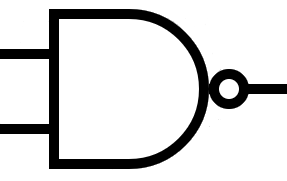
\includegraphics[scale=0.5]{img/schemes/NAND_symbol.png}
                \caption{Symbol bramki NAND}
                \label{fig:symbol_NAND}
            \end{figure}
        \item Wyrażenie algebraiczne:
            \begin{equation}
                \label{eq:NAND}
                Y = \overline{AB}
            \end{equation}
        \item Tabela prawdy:
        \begin{center}
            \label{tabela_prawdy:NAND}
            \begin{tabular}{|c|c|>{\columncolor[gray]{0.8}}c|}
                \hline
                A & B & Y \\
                \hline
                0 & 0 & 1 \\
                \hline
                0 & 1 & 1 \\
                \hline
                1 & 0 & 1 \\
                \hline
                1 & 1 & 0 \\
                \hline
            \end{tabular}
        \end{center}
 \end{itemize}
 
\section{Wzmacniacz sumujący - sumator napięć}

\begin{itemize}
    \item Schemat sumatora:
        \begin{figure}[H]
            \centering
            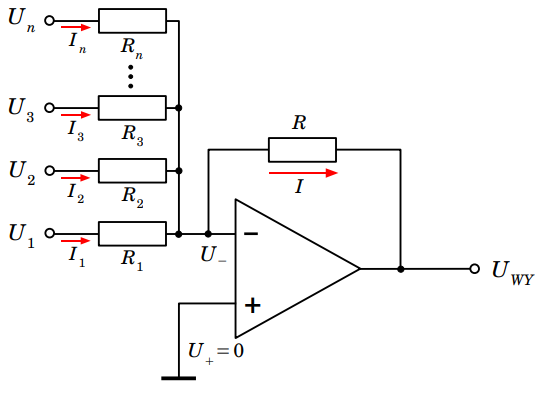
\includegraphics[scale=0.4]{img/schemes/sumator.png}
            \caption{Schemat sumatora}
            \label{fig:schemat_sumatora}
        \end{figure}
    \item Wzór na napięcie wyjściowe:
        \begin{gather}
            U_{wy} = -R(\dfrac{U_1}{R_1} + \dfrac{U_2}{R_2} + \dfrac{U_3}{R_3} + \dots + \dfrac{U_n}{R_n}) \\
            R_1 = R_2 = \dots = R \implies U_{wy} = -(U_1 + U_2 + \dots + U_n)
        \end{gather}
\end{itemize}

\section{Licznik}

\begin{itemize}
    \item Licznikem nazywamy układ cyfrowy służący do zliczania impulsów.
    \item Na wyjściu licznika pojawia się zakodowana binarnie liczba impulsów podanych na wejście zliczające. 
    \item Oprócz wejścia impulsów zliczanych, licznik posiada zazwyczaj wejście ustawiające stan początkowy (zerowanie licznika).
    \item Podstawowymi elementami liczników są przerzutniki T. Pojedynczy przerzutnik T pozwala na zliczanie 2 impulsów. 
    \item Najprostszy licznik można zbudować z szeregowo połączonych przerzutników T, z których każdy pod wpływem impulsu zegarowego zmienia swój stan na przeciwny do stanu poprzedniego.
    \begin{figure}[H]
        \centering
        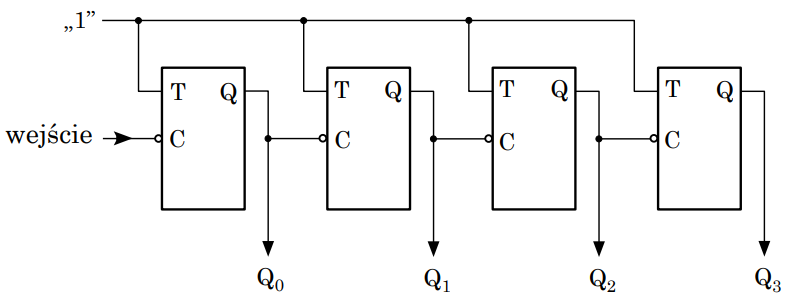
\includegraphics[width=0.8\textwidth]{img/schemes/schemat_licznika_4bitowego.png}
        \caption{Przykładowy licznik 4-bitowy}
        \label{licznik:przykladowy_licznik_4bitowy}
    \end{figure}
    \begin{figure}[H]
        \centering
        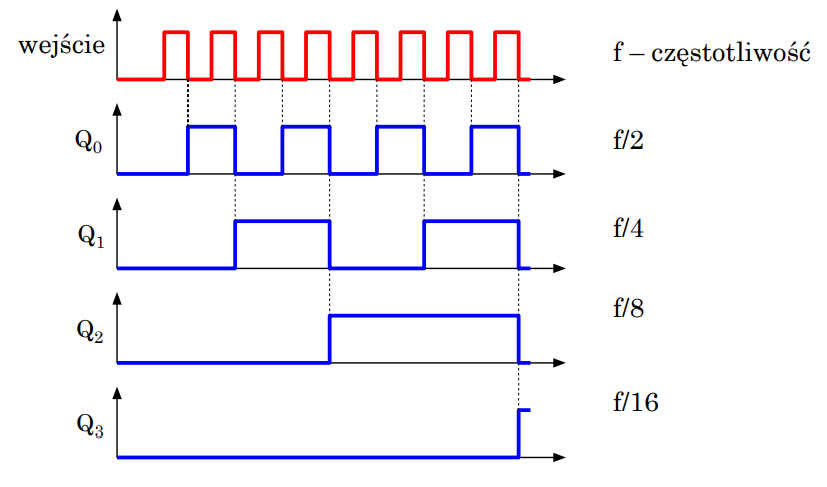
\includegraphics[width=0.8\textwidth]{img/schemes/licznik_przebieg.png}
        \caption{Przebieg czasowy licznika}
        \label{licznik:przebieg}
    \end{figure}
\end{itemize}
